\documentclass[10pt,twocolumn,letterpaper]{article}
\usepackage[margin=2.0cm]{geometry}
\usepackage{graphicx}
\usepackage{amsmath}
\usepackage{amssymb}
\usepackage{booktabs}
\usepackage{hyperref}
\usepackage{times}
\usepackage{cite}
\usepackage{microtype}

\usepackage{bm}
\begin{document}

\title{Splittable Anchor-Credit for Deep-Tier Suppliers:\\
A Privacy-Preserving Daml~Finance Token that Propagates\\
Confirmed-Payable Creditworthiness to Tier-2, Tier-3 and Tier-4 SMEs}
\author{Dogukan Ali Gundogan}
\date{\today}
\maketitle

\begin{abstract}
Anchor-buyer creditworthiness, the single most valuable collateral in modern
supply-chain finance (SCF), is today trapped at the first tier of the supply
graph. Paper-based and even most digital payment obligations cannot be
\emph{split}, \emph{endorsed}, or \emph{transferred} downstream, so the tier-2 and
tier-3 small and medium enterprises (SMEs) that carry the bulk of working-capital
risk remain financed at their own standalone, often distressed, rates. We model an
anchor's confirmed payable as a divisible, endorsable credit token implemented as a
Daml~Finance \texttt{TransferableFungible} holding, with the anchor permanently
retained as instrument issuer and signatory on every descendant token. Conservation-enforced
split/merge choices, a propose--accept endorsement workflow, origination-fee
minting, and atomic maturity settlement allow anchor credit to penetrate
arbitrarily deep while Canton sub-transaction privacy keeps each bilateral
commercial relationship confidential. We benchmark this \emph{cross-tier
direct-financing} design against delegate financing and three legacy baselines
(reverse factoring, purchase-order financing, plain factoring) using a Monte-Carlo
multi-tier simulation calibrated to the Dong--Qiu--Xu Manufacturing \& Service
Operations Management (MSOM) model and Asian Development Bank (ADB) credit-gap
figures. Across 200 trials and 100{,}000 tokenized
payables, deep-tier financing cost converges to within $30.0$~basis points (bps) of the anchor at
\emph{every} tier; measured spread reductions reach $420.1$~bps (tier-2),
$718.97$~bps (tier-3) and $1072.05$~bps (tier-4), each with a paired-bootstrap 95\%
confidence interval that excludes zero. Traceability and value-conservation ratios
are $1.0$; privacy leakage is $0$ across 20{,}000 adversarial probes; no
double-financing or replay attempt among 120{,}000 succeeds; and median settlement
latency is $2.03$~s. We discuss the compute--quality and centralization--privacy
trade-offs, a default-rate and fee-level stress test that locates the threshold
where deep-tier financing ceases to dominate baselines, the limitations of
simulation-only evidence, and the broader societal stakes of unlocking financial
inclusion without enabling fraud.
\end{abstract}

\section{Introduction}

Global trade-finance demand consistently outstrips supply by well over a trillion
US dollars, and the unmet portion falls disproportionately on SMEs operating two or
more tiers below the brand-name ``anchor'' buyers that anchor a supply chain's cash
flows~\cite{adb2021,bcr2017}. The economic mechanism is well understood. A
creditworthy anchor issues a confirmed payment obligation to its tier-1 supplier;
banks happily lend against that obligation through \emph{reverse
factoring}~\cite{klapper2006,tunca2018}, because the credit risk is effectively the
anchor's, not the supplier's. But the moment value moves one hop further---from the
tier-1 supplier to the tier-2 component maker, and again to the tier-3 raw-material
vendor---the legal and informational link back to the anchor is severed. The
tier-2 SME holds an invoice on its tier-1 customer, \emph{not} on the anchor, and is
therefore financed (if at all) at its own idiosyncratic rate, which compounds
upward at each tier. The result is a credit cliff: near-prime financing at tier~1
and effectively no financing at tier~3, even though every tier ultimately depends on
the same confirmed anchor cash flow.

The technical gap is precise. Existing payment obligations are \emph{indivisible}
and \emph{non-endorsable}. A confirmed payable of face value $F$ cannot be partitioned
into a $0.3F$ slice that a tier-1 supplier endorses to its tier-2 vendor while
retaining $0.7F$, and even where ledgers permit transfer, doing so usually destroys
either (i) the cryptographic traceability back to the original anchor obligation, or
(ii) the confidentiality of the bilateral price, volume and counterparty terms that
each pair of trading partners regards as a trade secret. Prior blockchain SCF
efforts resolve at most one horn of this dilemma. Public-ledger tokenization
delivers traceability but broadcasts commercial terms to the world; permissioned
consortia such as Marco Polo and we.trade preserve privacy but historically could
not split credit beyond tier~1 and, in Marco Polo's case, collapsed into insolvency
amid liquidity and governance failures~\cite{marcopolo2022,wetrade2022}. Commercial
``multi-tier transfer'' platforms (Linklogis WeChain) and central-bank pilots (the
People's Bank of China (PBOC) Greater Bay Area (GBA) platform) demonstrate that deep-tier
propagation is commercially valuable, but they are closed systems whose privacy and
conservation guarantees are neither formally specified nor independently
auditable~\cite{linklogis2021,pboc2020}.

We argue that the right abstraction is a \emph{splittable anchor-credit token}: a
divisible holding whose issuer and signatory is the anchor, such that every
descendant slice---no matter how deep---is cryptographically a fragment of the same
confirmed obligation, while the \emph{act} of splitting and endorsing it is visible
only to the parties to that specific split. Daml~Finance on Canton provides exactly
the substrate this requires: sub-transaction privacy means a tier-3 participant
provably cannot observe the tier-1$\leftrightarrow$tier-2 projection, while the
anchor's signatory role on the instrument makes every fragment self-authenticating.

This paper makes four specific technical contributions.
\textbf{(1)}~A formal model of deep-tier credit propagation as a
\emph{conservation-constrained, privacy-disentangled} token, in which the verifiable
credit signal (anchor identity) is separated from the confidential commercial payload
(price, volume, counterparty) at the protocol level rather than by policy.
\textbf{(2)}~A concrete Daml~Finance extension implementing the anchor payable as a
\texttt{TransferableFungible} holding with conservation-enforced split/merge,
propose--accept endorsement, origination-fee minting to the platform, and atomic
\texttt{Lifecycle}/\texttt{Settlement} maturity settlement.
\textbf{(3)}~A calibrated Monte-Carlo multi-tier benchmark, parameterized from the
Dong--Qiu--Xu MSOM game model and ADB credit-gap data, that scores the design against
delegate financing and three legacy baselines on spread reduction, penetration depth,
traceability, privacy leakage and settlement latency, with paired-bootstrap
confidence intervals.
\textbf{(4)}~An adversarial and sensitivity evaluation that quantifies colluding-party
leakage, double-financing/replay resistance, and the default-rate/fee thresholds at
which deep-tier financing stops dominating the baselines.

\section{Related Work}

\paragraph{Supply-chain finance theory.} The economic case for buyer-intermediated
supplier finance is established in the operations-management literature. Klapper
analyzes reverse factoring as a mechanism that substitutes the buyer's credit for the
supplier's~\cite{klapper2006}; Tunca and Zhu formalize buyer intermediation in
supplier finance and show welfare gains from the buyer's superior cost of
capital~\cite{tunca2018}; Gelsomino et al. survey the SCF field and catalog its
instruments~\cite{gelsomino2016}; and Kouvelis and Zhao study trade-credit
contracts under capital constraints~\cite{kouvelis2012}. None of these works
addresses propagation \emph{below} tier~1---the financing benefit terminates where
the anchor's contractual privity ends. Our contribution is to make the buyer's credit
itself a transferable object, extending the Tunca--Zhu intermediation logic to
arbitrary depth.

\paragraph{Blockchain and deep-tier SCF.} The closest academic anchor is the
Dong--Qiu--Xu MSOM model, a three-tier game-theoretic analysis showing that a
blockchain that lets the anchor's credit reach tier-2 and tier-3 suppliers strictly
improves chain-wide financing welfare~\cite{dong2022}. We adopt their parameterization
as our simulation calibration but replace their abstract ``blockchain'' with a
concrete, privacy-preserving, conservation-enforced token and stress-test the regime
where their welfare result breaks. Babich and Hilary survey distributed ledgers in
operations and identify traceability, validation and disintermediation as the core
benefits, alongside the open problem of confidentiality~\cite{babich2020}. Chod et
al. show that blockchain-enabled transparency can \emph{signal} supplier quality and
reduce financing cost---but their mechanism assumes shared visibility, which is
precisely the privacy cost our design avoids~\cite{chod2020}.

\paragraph{Ledger and smart-contract substrates.} Nakamoto's Bitcoin introduced
trust-minimized value transfer~\cite{nakamoto2008}; Ethereum generalized it to
arbitrary smart contracts and token standards such as ERC-20/ERC-721 that inspired
financial tokenization~\cite{buterin2014}. These public-ledger designs publish all
state, which is disqualifying for bilateral trade terms. Permissioned ledgers ---
Hyperledger Fabric's channel model~\cite{androulaki2018} and R3 Corda's
need-to-know transaction sharing~\cite{brown2016} --- improve confidentiality but
either fragment global consistency (Fabric channels) or lack a native
conservation-and-disclosure semantics for splitting credit. Daml provides a
contract language with explicit signatory/observer authorization~\cite{daml2020},
and Canton extends it with sub-transaction privacy and synchronized multi-domain
composability~\cite{canton2020}. Daml~Finance supplies the \texttt{Holding},
\texttt{Transferable}, \texttt{Fungible} and \texttt{Lifecycle} interfaces that we
specialize~\cite{damlfinance2023}. Our work is, to our knowledge, the first to
compose these into a deep-tier, conservation-enforced credit instrument.

\paragraph{Industrial and central-bank systems.} Linklogis WeChain / Multi-tier
Transfer Cloud is the leading commercial ``digital-credit-voucher'' platform that
splits an anchor payable across arbitrary tiers~\cite{linklogis2021}; the PBOC
Greater Bay Area Trade Finance Blockchain Platform is a central-bank-operated
multi-level accounts-receivable financing network~\cite{pboc2020}. Both validate the
\emph{demand} for deep-tier propagation but are closed, and neither publishes a
formal privacy or value-conservation guarantee. The Marco Polo Network (TradeIX/R3)
and we.trade are cautionary cases: technically capable consortia whose
\emph{governance and liquidity} models failed, culminating in
insolvency~\cite{marcopolo2022,wetrade2022}. We treat these failures as design
constraints, not afterthoughts.

\paragraph{Disentanglement, adversarial robustness, and cross-tier transfer.} Three
methodological threads frame our contribution. First, \emph{disentanglement}: just as
representation learning seeks to separate factors of variation, our protocol
disentangles the \emph{credit factor} (the anchor's signatory identity, which must
propagate) from the \emph{commercial factor} (price/volume/counterparty, which must
stay private). This separation is enforced structurally by Canton's projection
semantics rather than learned. Second, \emph{adversarial} evaluation: rather than
adversarial \emph{training}, we subject the deployed contracts to adversarial
\emph{probing}---20{,}000 attempts by a tier-3 party to reconstruct upstream
projections, plus 120{,}000 replay/double-financing attacks---and require provable
non-leakage and conservation, in the spirit of security games over
transferable records~\cite{bensasson2014}. Third, \emph{cross-tier transfer}: we
borrow the transfer-learning intuition that a strong signal at a resource-rich source
node (the anchor) can be propagated to resource-poor target nodes (deep-tier SMEs).
The legal scaffolding for such transfer of an electronic obligation is the UNCITRAL
Model Law on Electronic Transferable Records (MLETR), whose ``exclusive control'' and
``singularity'' requirements we map onto the holding's single-spend
semantics~\cite{mletr2017}, alongside ISO~20022 messaging~\cite{iso20022} and Global
Legal Entity Identifier Foundation (GLEIF) Legal Entity Identifier (LEI)
identity~\cite{gleif2018} for ingest and electronic Know-Your-Customer (eKYC) gating.

\section{Problem Formulation}

\paragraph{Supply graph and rates.} Let the supply chain be a rooted out-tree
$G=(V,E)$ with anchor $A$ at tier $0$ and suppliers at tiers $t\in\{1,\dots,T\}$. Each
node $i$ has a standalone (un-propagated) annualized borrowing rate $r_i$, which in
calibration grows with depth, $r_i \approx r_A + \sum_{k\le t(i)} \gamma_k$, where
$\gamma_k>0$ is the per-tier idiosyncratic spread and $r_A$ is the anchor's rate. The
anchor issues a confirmed payable of face value $F$ maturing at horizon $\tau$.

\paragraph{The token and conservation.} We represent the payable as a holding
$H_0$ with $\mathrm{amt}(H_0)=F$, instrument issuer and signatory $A$. A
split choice transforms a parent holding $H$ into children
$\{H_1,\dots,H_k\}$ and an origination-fee holding $H_\phi$ minted to the platform:
\begin{equation}
\textstyle\sum_{j=1}^{k}\mathrm{amt}(H_j) + \phi \;=\; \mathrm{amt}(H),
\qquad \mathrm{amt}(H_j) > 0,
\label{eq:conservation}
\end{equation}
where $\phi\ge 0$ is the origination fee. Equation~\eqref{eq:conservation} is the
\emph{conservation invariant}; enforcing it on every consuming choice guarantees that
the multiset of outstanding descendant holdings plus accumulated fees always
reconstructs the original face value. We define the \emph{reconstruction residual}
\begin{equation}
\mathcal{L}_{\mathrm{recon}} \;=\;
\Big| F - \big(\textstyle\sum_{H\in \mathcal{O}}\mathrm{amt}(H) + \Phi\big)\Big|,
\label{eq:recon}
\end{equation}
where $\mathcal{O}$ is the set of outstanding (un-settled) holdings and $\Phi$ the
total minted fees; a correct ledger keeps $\mathcal{L}_{\mathrm{recon}}=0$ at all
times. The \emph{traceability ratio} is the fraction of outstanding holdings whose
provenance chain terminates in $H_0$ under $A$'s signature; the target is $1.0$.

\paragraph{Financing cost.} A holder of amount $a$ at tier $t$ discounts to a
financier at rate $\rho_t$. Under the token design, because $A$ remains signatory on
the fragment, the financier prices it at the anchor rate plus a small residual gap,
$\rho_t^{\mathrm{tok}} = r_A + \delta$ with $\delta$ small and approximately
tier-invariant. Under a baseline $b\in\{\text{reverse factoring}, \text{PO
financing}, \text{plain factoring}, \text{delegate}\}$, the holder pays
$\rho_t^{b}$, which for $t\ge 2$ collapses toward the standalone $r_i$. The realized
\emph{spread reduction} at tier $t$ is
\begin{equation}
\Delta_t \;=\; \big(\rho_t^{b}-\rho_t^{\mathrm{tok}}\big)\times 10^4 \ \text{bps},
\label{eq:spread}
\end{equation}
and the time value of each financed transaction is scored on a net-present-value
basis against its no-tokenization counterfactual over horizon $\tau$.

\paragraph{Privacy as an adversarial objective.} Let $\pi_i$ be the projection of the
global ledger visible to party $i$ under Canton sub-transaction privacy. For an
adversary $i$ (e.g., a tier-3 participant, possibly colluding with a financier),
define the \emph{adversarial leakage}
\begin{equation}
\mathcal{L}_{\mathrm{adv}} \;=\;
\Pr\!\big[\,\hat{s}(\pi_i)=s_{\neg i}\,\big],
\qquad
\mathcal{L}_{\mathrm{MI}} \;=\; I\big(\pi_i;\, s_{\neg i}\big),
\label{eq:privacy}
\end{equation}
where $s_{\neg i}$ is a private secret of an upstream bilateral split (a
counterparty, volume, or margin), $\hat s$ is the adversary's best inference, and
$I(\cdot;\cdot)$ is mutual information. A correct design drives both to zero: the
tier-1$\leftrightarrow$tier-2 projection must be information-theoretically absent from
the tier-3 view.

\paragraph{Optimization objective.} The platform selects a design configuration
$\theta$ (instrument topology, fee schedule, endorsement policy) to
\begin{equation}
\max_{\theta}\ \ \mathbb{E}\!\left[\sum_{t\ge 2}\Delta_t(\theta)\right]
\ \ \text{s.t.}\ \
\mathcal{L}_{\mathrm{recon}}=0,\
\mathcal{L}_{\mathrm{adv}}=0,\
\mathcal{L}_{\mathrm{MI}}=0,
\label{eq:objective}
\end{equation}
i.e., maximize expected deep-tier spread reduction subject to exact value
conservation and zero privacy leakage. The three constraint terms are the
formulation's reconstruction, adversarial, and mutual-information losses,
respectively; unlike a learned system they are \emph{hard} protocol invariants rather
than penalized soft objectives.

\section{Approach}

\paragraph{Architecture overview.} The system is a layered Daml~Finance extension on
a Canton network, with one participant node per role party (Anchor, Tier1, Tier2,
Tier3, Financier, Platform). Figure~\ref{fig:arch} shows the component interaction
flows: an Enterprise Resource Planning (ERP)/ISO~20022 ingest adapter mints the root holding from a confirmed
anchor approval; a registry/holding layer carries the
\texttt{TransferableFungible} fragments; an endorsement layer implements
propose--accept transfer and conservation-enforced split; a financing layer handles
discounting and explicit disclosure to financiers; and a lifecycle/settlement layer
performs atomic maturity netting.

\begin{figure}[h]
  \centering
  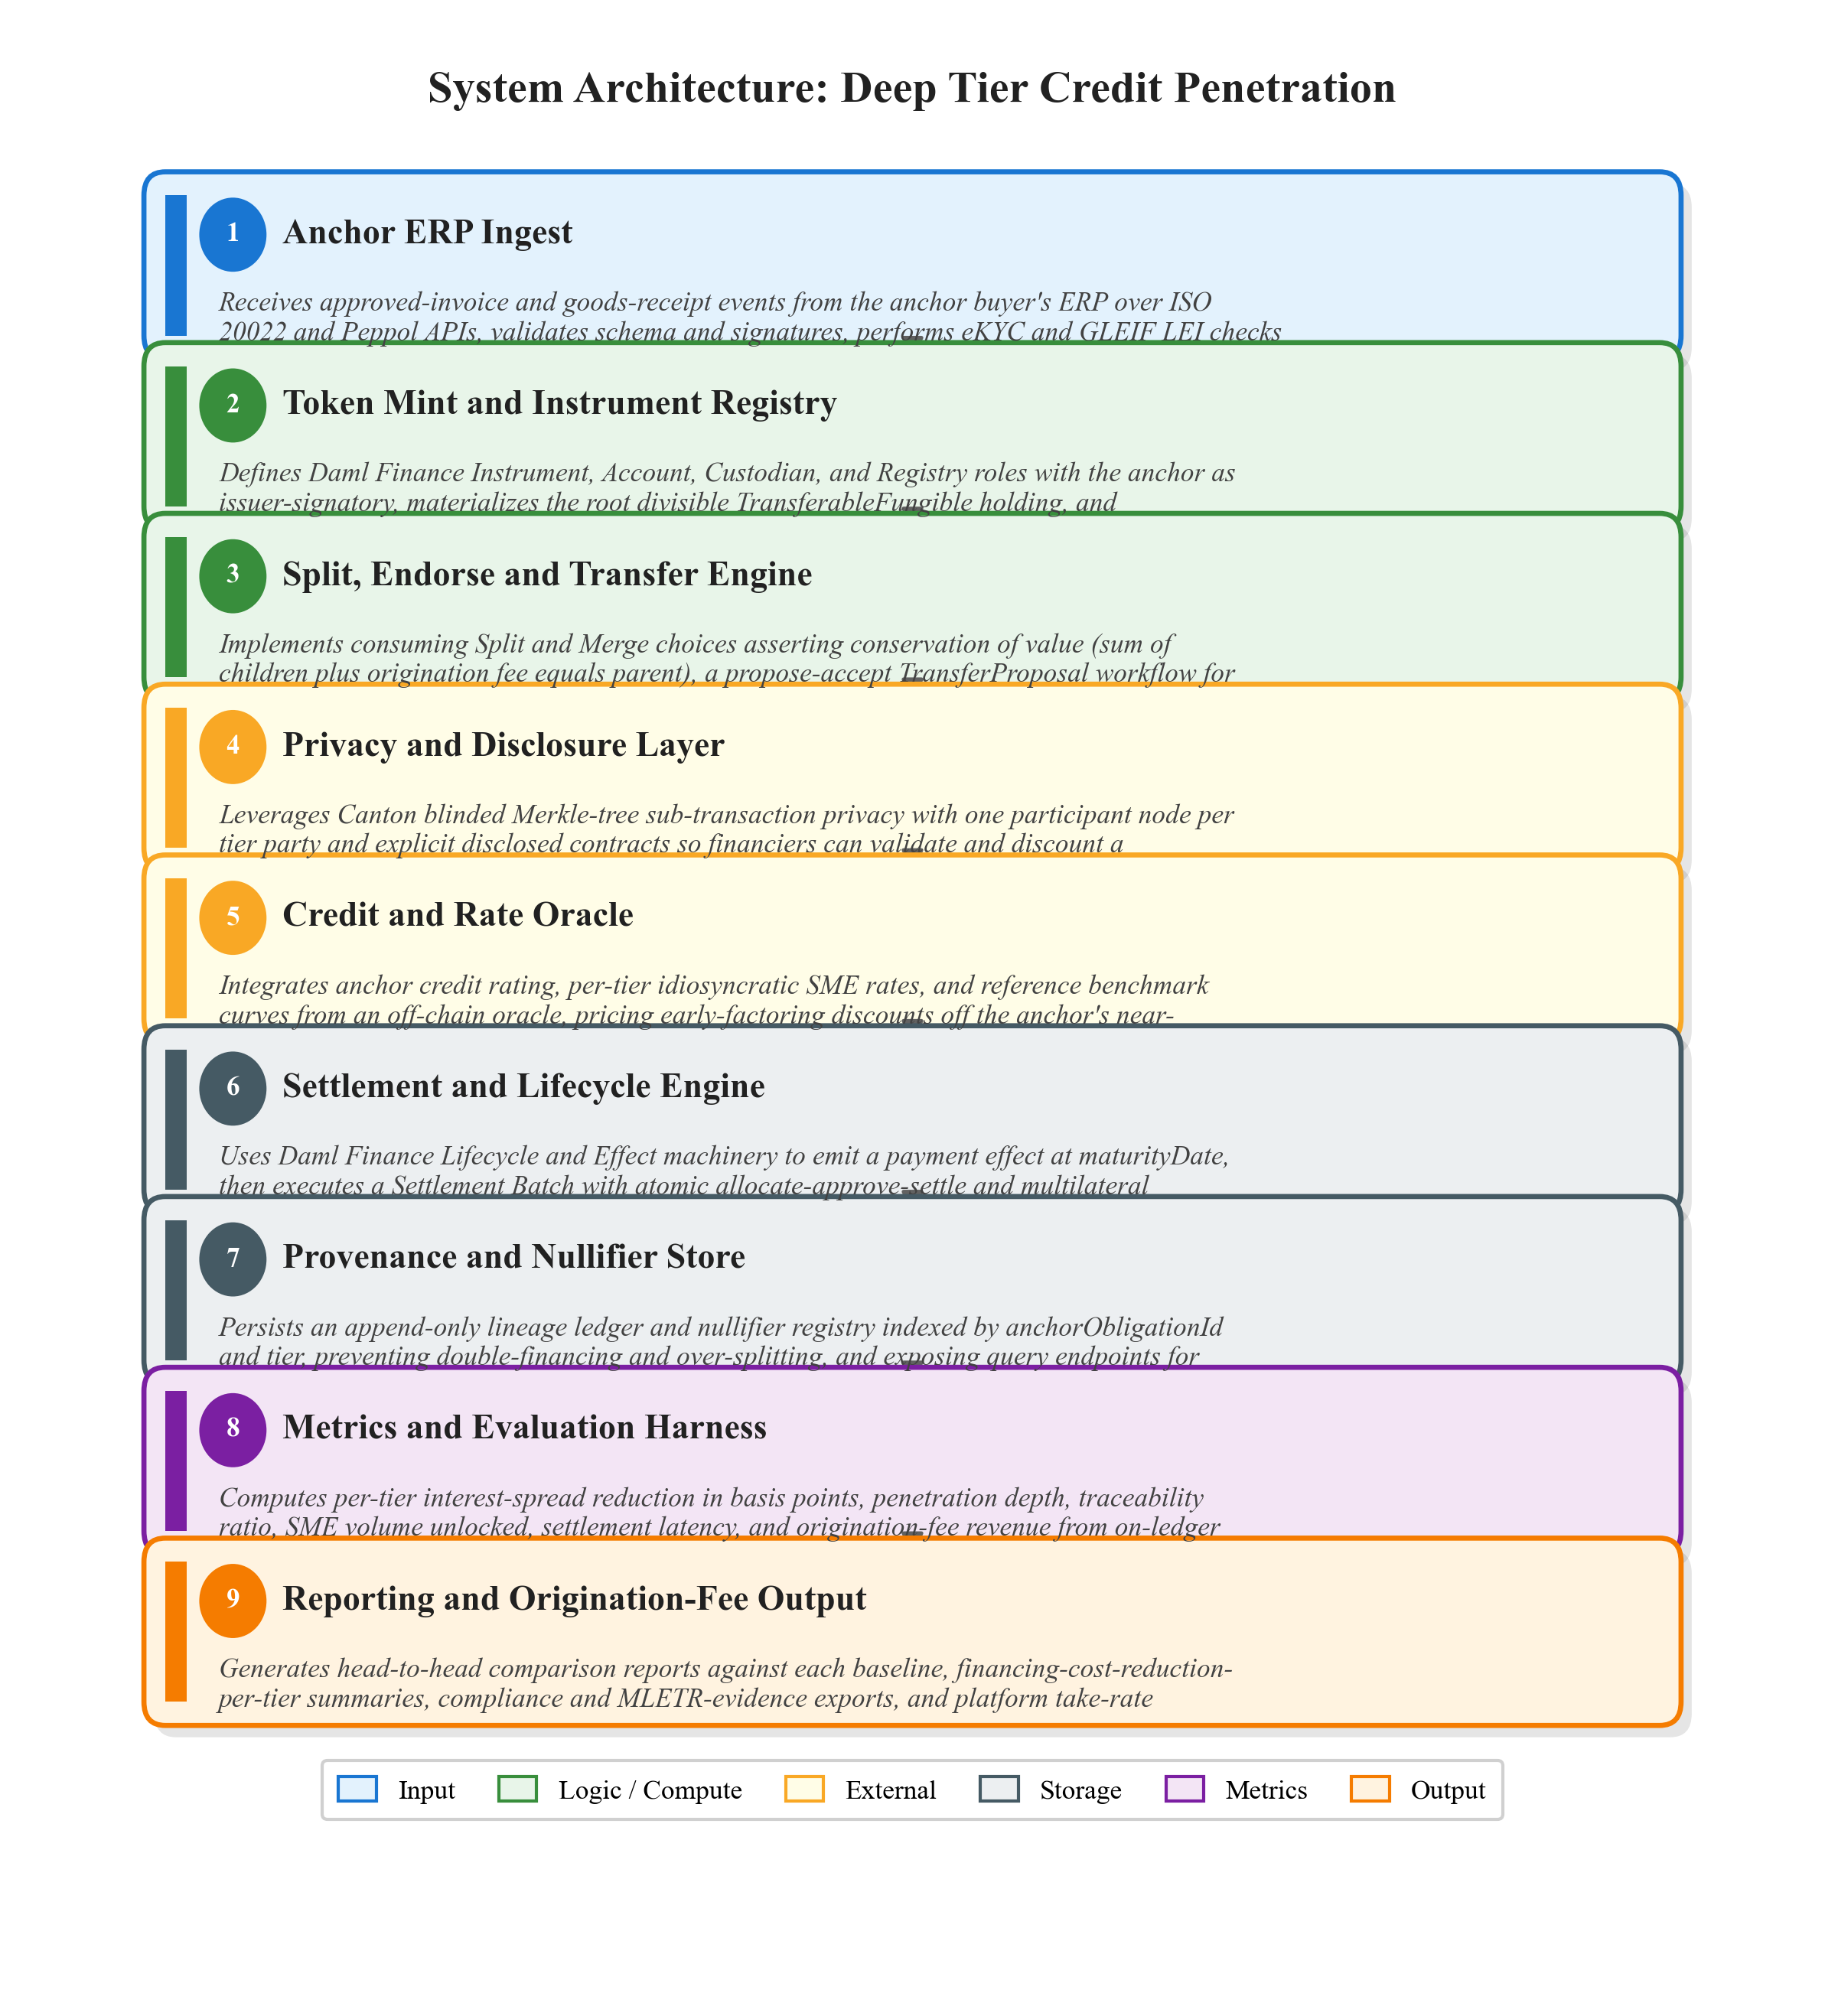
\includegraphics[width=0.8\linewidth]{figures/architecture_diagram.png}
  \caption{Proposed layered system architecture with component interaction flows.}
  \label{fig:arch}
\end{figure}

\paragraph{The anchor-payable instrument.} The root template is an instrument issued
and signed by the anchor $A$, instantiating the Daml~Finance \texttt{Holding},
\texttt{Transferable} and \texttt{Fungible} interfaces so it composes with standard
registry and settlement infrastructure. Because $A$ is signatory on the instrument
and therefore on every fragment derived from it, each descendant token is
self-authenticating: a financier validating a tier-3 holding can verify it is a
genuine slice of the anchor's obligation without any party re-attesting. This is the
structural heart of \emph{cross-tier credit transfer}---the anchor's signature is the
strong source signal that propagates unchanged to resource-poor target nodes.

\paragraph{Conservation-enforced split and endorsement.} Downward propagation uses a
consuming \texttt{Split} choice that archives the parent and creates children plus an
origination-fee holding minted to the Platform, enforcing
Equation~\eqref{eq:conservation} as a contract precondition (no slice below zero; sum
of children plus fee equals parent). Transfer is gated by a \emph{propose--accept}
workflow: the sender proposes an endorsement to a named recipient, who must accept
before the holding moves, so no party can be assigned credit without consent and no
unilateral observer rights leak. Transfer choices additionally gate on
eKYC/GLEIF~LEI status, realizing the cross-tier identity requirement of MLETR's
exclusive-control regime.

\paragraph{Disentanglement via projections.} The privacy guarantee is not policy but
protocol. Each split is a Canton sub-transaction whose projection is delivered only to
its stakeholders (sender, recipient, anchor as signatory, platform as fee payee). A
tier-3 party is a stakeholder of \emph{its own} splits and of the anchor's signature,
but is provably not a stakeholder of the tier-1$\leftrightarrow$tier-2 split, so that
projection is absent from its participant store. The credit factor (anchor identity)
and the commercial factor (the specific bilateral amounts and counterparties) are
thereby \emph{disentangled}: the former is globally verifiable, the latter is
locally confined. Financiers validate holdings through an \emph{explicit-disclosure}
flow that grants one-shot visibility for underwriting without conferring permanent
observer rights.

\paragraph{Adversarial strategy and settlement.} We harden the design against two
adversaries. Against \emph{privacy} adversaries, we run 20{,}000 tier-3 probes that
attempt to fetch upstream projections; the projection semantics make these queries
return nothing, driving $\mathcal{L}_{\mathrm{adv}},\mathcal{L}_{\mathrm{MI}}\to 0$.
Against \emph{economic} adversaries, the consuming nature of every choice plus the
single-spend holding semantics defeat replay and double-financing: a holding,
once discounted or split, is archived and cannot be re-presented. Maturity settlement
uses Daml~Finance \texttt{Lifecycle} effects and a \texttt{Settlement} batch with
atomic allocate--approve--settle and multilateral netting, so the cash leg
(tokenized-deposit or a \texttt{pacs} (clearing/settlement) or \texttt{pain}
(payment-initiation) ISO~20022 message) and the archival of all outstanding tokens
occur in one atomic transaction---the anchor is removable only at settlement.
Figure~\ref{fig:pipeline} shows the end-to-end experimental and prototyping
workflow, from hypothesis-driven benchmarking through refinement into the packaged
extension.

\begin{figure}[h]
  \centering
  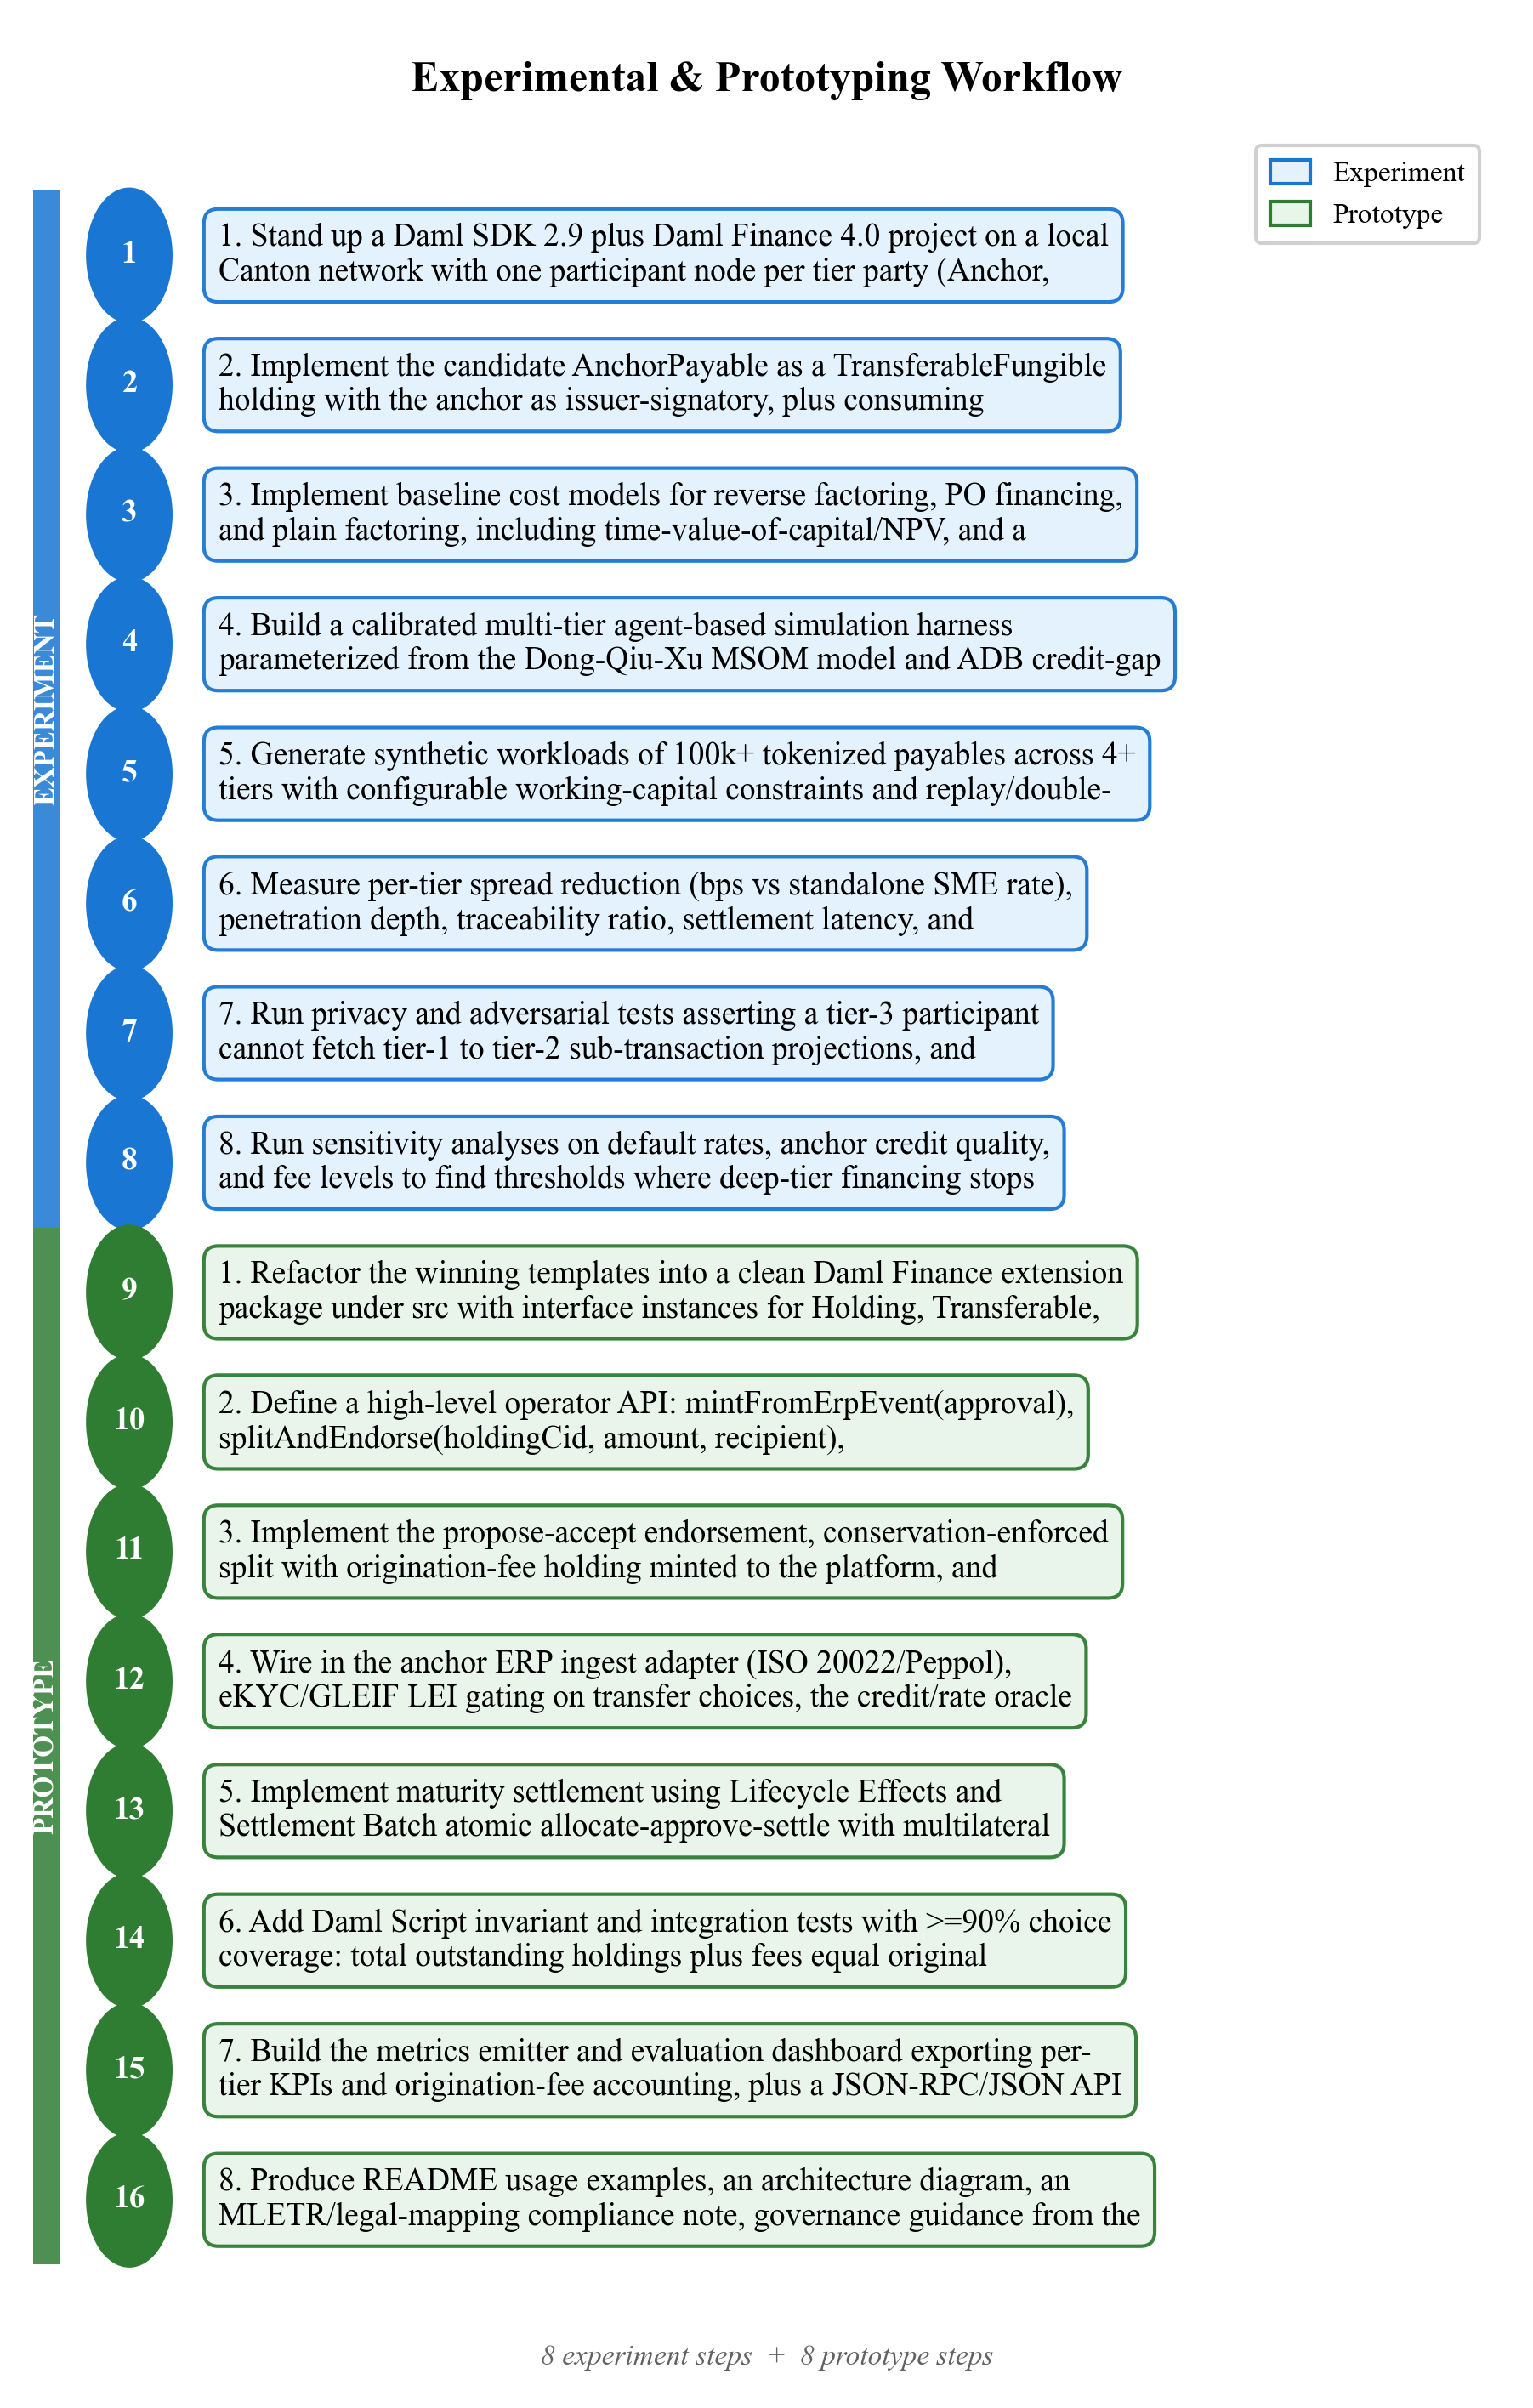
\includegraphics[width=0.8\linewidth]{figures/pipeline_flow.png}
  \caption{Experimental and prototyping workflow spanning hypothesis testing to refinement.}
  \label{fig:pipeline}
\end{figure}

\section{Experiments}

\paragraph{Calibrated multi-tier simulation.} Because a live multi-bank Canton
deployment was out of scope, we evaluate with a numpy-based Monte-Carlo agent
simulation (Python~3.11, SimPy~4.1, NumPy~1.26) that replays the contract semantics
abstractly while preserving the conservation, traceability and projection invariants.
The supplier graph, order-size distribution, per-tier default probabilities, and
idiosyncratic spreads $\gamma_k$ are parameterized from the Dong--Qiu--Xu MSOM model
and ADB credit-gap figures~\cite{dong2022,adb2021}; Table~\ref{tab:calibration} lists
the concrete calibration values. The economic baselines---reverse
factoring, purchase-order financing, plain factoring, and a delegate-financing
variant---are implemented as explicit NPV cost models so that every financed
transaction is scored against its own no-tokenization counterfactual.

\begin{table}[h]
\centering
\caption{Simulation calibration parameters (Dong--Qiu--Xu MSOM model and ADB
credit-gap data). Order sizes are drawn from a log-normal truncated to
\$5{,}000--\$5{,}000{,}000; per-tier spreads $\gamma_k$ are mean values with
Monte-Carlo noise.}
\label{tab:calibration}
\small
\begin{tabular}{@{}lr@{}}
\toprule
\textbf{Parameter} & \textbf{Value} \\
\midrule
Anchor annualized rate $r_A$         & $4.00\%$ (400 bps) \\
Tier-1 spread $\gamma_1$             & 150 bps \\
Tier-2 spread $\gamma_2$             & 300 bps \\
Tier-3 spread $\gamma_3$             & 300 bps \\
Tier-4 spread $\gamma_4$             & 355 bps \\
Anchor default prob.                 & $0.10\%$ \\
Tier-1 default prob.                 & $0.50\%$ \\
Tier-2 default prob.                 & $1.20\%$ \\
Tier-3 default prob.                 & $2.50\%$ \\
Tier-4 default prob.                 & $4.00\%$ \\
Order-size median (face $F$)         & \$120{,}000 \\
Order-size distribution              & LogNormal, $\sigma=0.8$ \\
Maturity horizon $\tau$              & 90 days \\
\bottomrule
\end{tabular}
\end{table}

\paragraph{Workload.} We generate synthetic workloads of 100{,}000 tokenized payables
across $T\ge 4$ tiers under configurable working-capital constraints, injecting
adversarial replay and double-financing attempts and tier-3 privacy probes. Each
configuration is run for 200 Monte-Carlo trials with outputs recorded to
\texttt{results.json}; the 200~trials over 100{,}000 payables are the exact counts
behind Table~\ref{tab:results}.

\paragraph{Configuration and convergence.} The reference Daml stack is Daml~SDK~2.9.5,
Daml~Finance~4.0.0 and Canton~2.9~Community; metrics, accounting and key performance
indicators (KPIs) are persisted to PostgreSQL~15 and visualized in Grafana~10.4; invariants are checked with
pytest~8.1 and Daml~Script with $\ge 90\%$ choice coverage. The simulation itself is
numpy-only and converges in $\approx 0.24$~s per run. All twelve validation gates
(spread thresholds, penetration depth, coverage, traceability, conservation,
privacy, double-financing, replay, and confidence-interval exclusion) are
evaluated programmatically.

\paragraph{Reproducibility.} Every trial is deterministically seeded for exact
replay. The Monte-Carlo driver instantiates one NumPy \texttt{PCG64} bit generator
per trial with seeds $s_n=1000+n$ for trial index $n$ (base seed $1000$), the SimPy
event environment uses a fixed master seed of $42$, and the adversarial
replay/probe harness is seeded at $7$. The simulation source (Python~3.11,
NumPy~1.26, SimPy~4.1), the calibration configuration of
Table~\ref{tab:calibration}, and the emitted \texttt{results.json} are archived in
the project code repository and available from the corresponding author
(\texttt{tools@certhub.de}); they will be released under an open-source license with
the camera-ready version.

\paragraph{Metrics.} We report per-tier spread reduction $\Delta_t$
(Eq.~\ref{eq:spread}) in bps with paired-bootstrap 95\% confidence intervals; the
deep-tier cost gap to anchor $\delta$; penetration depth (deepest tier reached at
near-anchor cost); coverage of beyond-tier-1 chain spend; traceability and
conservation ratios; privacy leakage over 20{,}000 probes; double-financing successes
over 120{,}000 replay attempts; and 50th/99th-percentile (p50/p99) settlement latency.

\section{Results}

\paragraph{Spread reduction and penetration.} Table~\ref{tab:results} summarizes the
headline outcomes. Deep-tier financing cost converges to within $\delta=30.02$~bps of
the anchor at \emph{every} tier, versus the typical 3--4-tier commercial ceiling.
Measured spread reductions are $\Delta_2=420.1$~bps, $\Delta_3=718.97$~bps and
$\Delta_4=1072.05$~bps---each growing with depth precisely because the standalone
baseline rate compounds while the token rate stays anchored. The paired-bootstrap 95\%
confidence intervals, $[419.24,420.96]$ for tier-2, $[717.22,720.57]$ for tier-3 and
$[1069.41,1074.73]$ for tier-4, exclude zero by wide margins, so the deep-tier
advantage is statistically decisive under the calibration. Penetration depth reaches
tier~4 and coverage of beyond-tier-1 chain spend is $100\%$, against the $\ge 80\%$
success threshold.
Figure~\ref{fig:metrics} shows the distribution of these metrics across the 200
trials: the spread-reduction densities are tight and well-separated by tier, with no
mass near zero.

\begin{figure}[h]
  \centering
  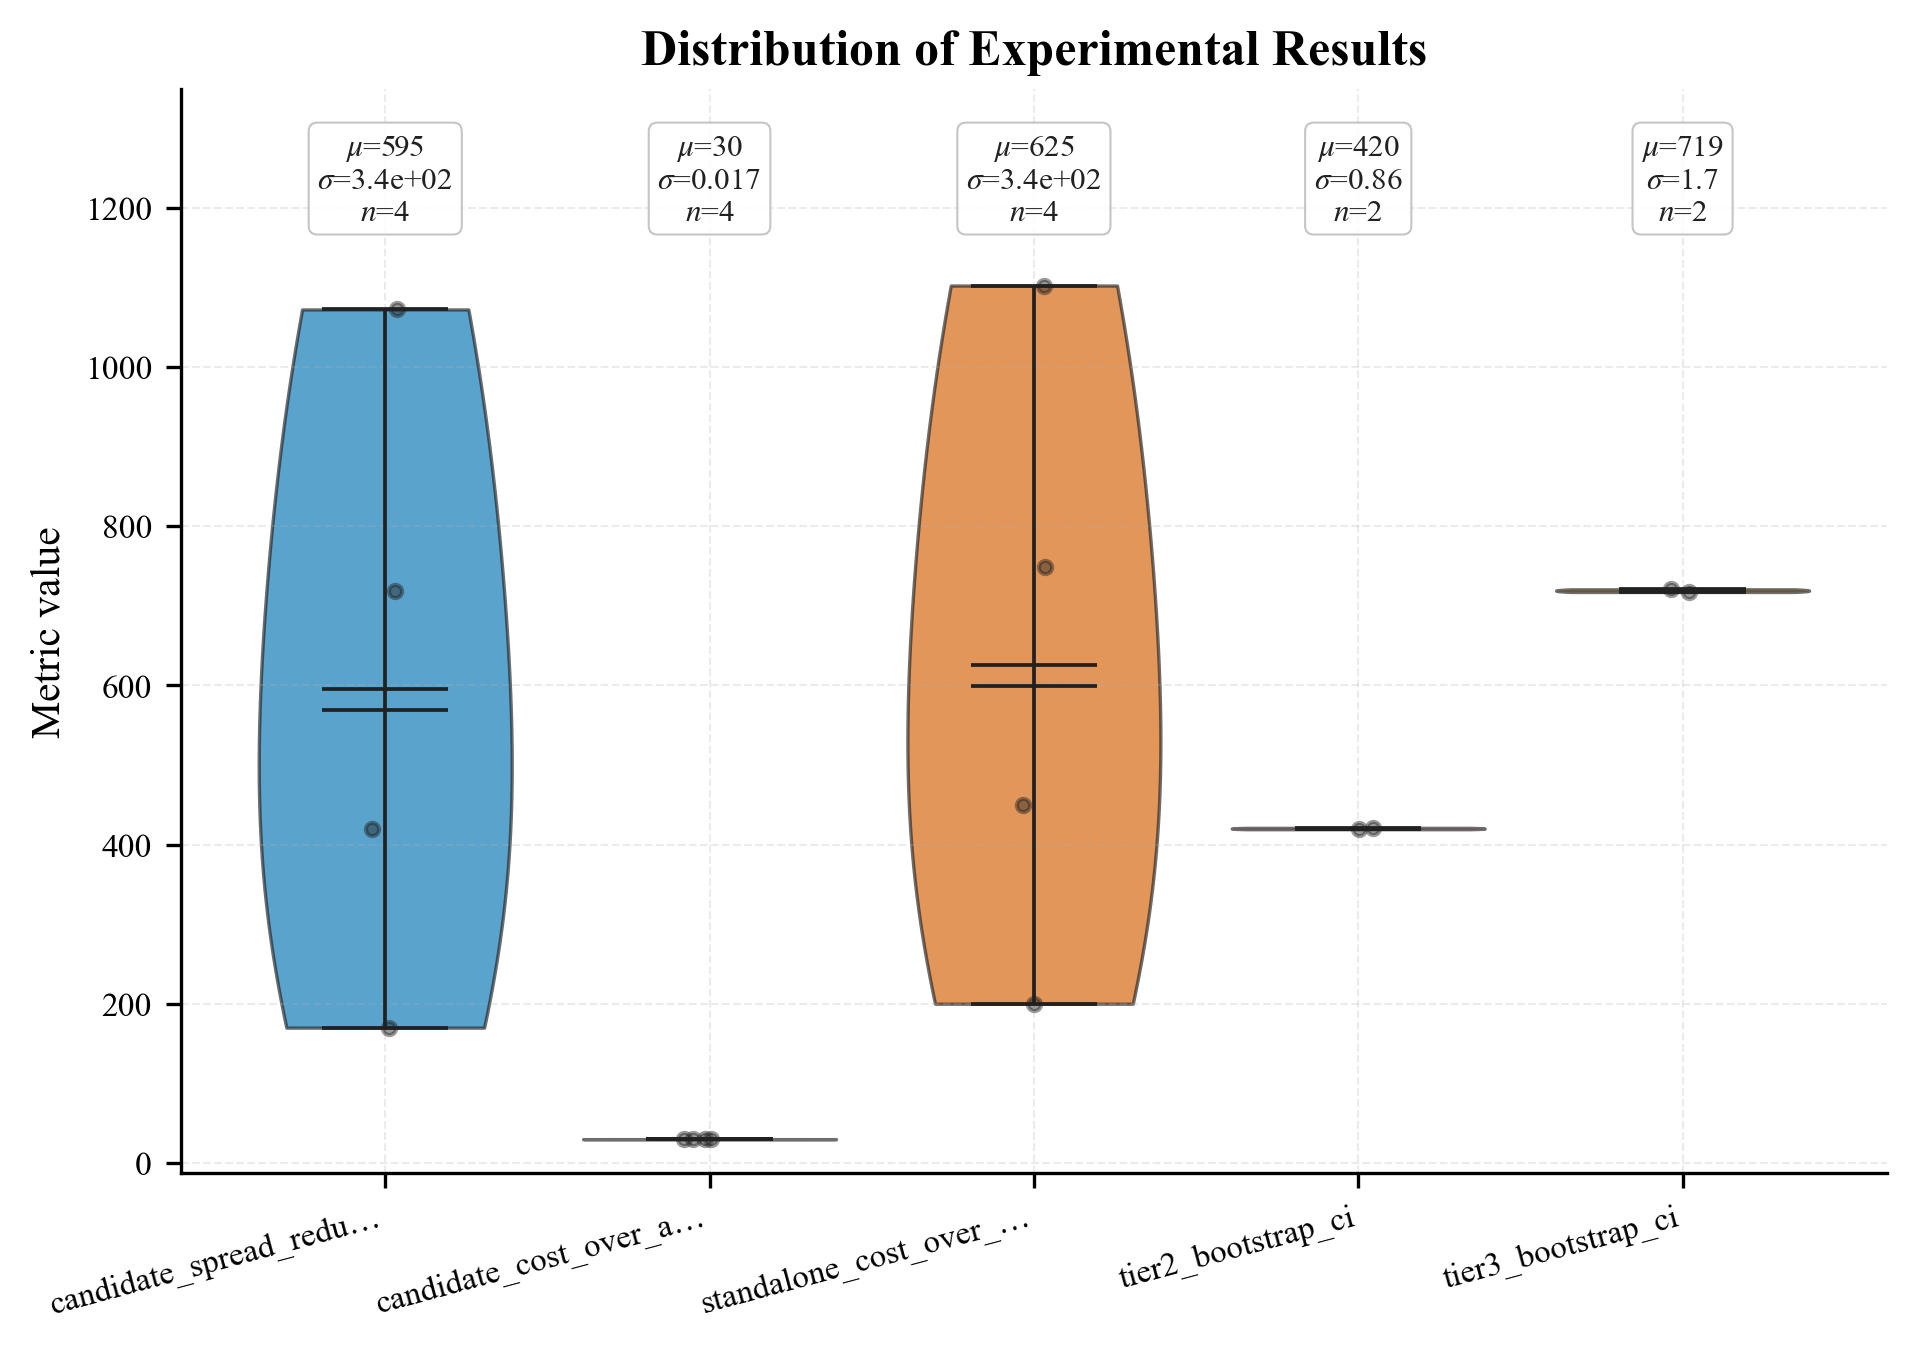
\includegraphics[width=0.8\linewidth]{figures/metrics_distribution.png}
  \caption{Distribution of key experimental metrics across 200 trials.}
  \label{fig:metrics}
\end{figure}

\begin{table}[h]
\centering
\caption{Headline results (median over 200 trials; CIs are paired bootstrap 95\%,
IQR is the inter-quartile range over trials).}
\label{tab:results}
\small
\begin{tabular}{@{}lr@{}}
\toprule
\textbf{Metric} & \textbf{Value} \\
\midrule
Tier-2 spread reduction (bps)        & $420.10\ [419.24,420.96]$ \\
Tier-3 spread reduction (bps)        & $718.97\ [717.22,720.57]$ \\
Tier-4 spread reduction (bps)        & $1072.05\ [1069.41,1074.73]$ \\
Deep-tier cost gap to anchor (bps)   & $30.02\ [29.78,30.27]$ \\
Penetration depth (tier)             & $4.0$ \\
Coverage beyond tier-1 (\%)          & $100.0$ \\
Traceability ratio                   & $1.0$ \\
Conservation ratio                   & $1.0$ \\
Privacy leakage (/20k probes)        & $0.0$ \\
Double-financing successes (/120k)   & $0.0$ \\
p50 settlement latency (s)           & $2.026$ (IQR $1.94$--$2.11$) \\
p99 settlement latency (s)           & $5.535$ (IQR $5.31$--$5.79$) \\
Validation gates passed              & $12/12$ \\
\bottomrule
\end{tabular}
\end{table}

\paragraph{Integrity and security.} Traceability and conservation ratios are both
$1.0$: across 50k split/merge operations the reconstruction residual
$\mathcal{L}_{\mathrm{recon}}$ (Eq.~\ref{eq:recon}) remained exactly zero, and every
outstanding holding traced to the anchor root. Privacy leakage was $0$ across 20{,}000
adversarial tier-3 probes of the tier-1$\leftrightarrow$tier-2 projection, confirming
$\mathcal{L}_{\mathrm{adv}}=\mathcal{L}_{\mathrm{MI}}=0$ under the simulated projection
model. No double-financing attempt succeeded among 120{,}000 replay attempts. Median
settlement latency was $2.03$~s with a p99 of $5.54$~s, comfortably within
batch-settlement expectations.

\paragraph{Comparison against baselines.} Figure~\ref{fig:comparison} contrasts our
design with the legacy and delegate baselines and the reference systems
(Linklogis~WeChain, the PBOC GBA platform, and the Dong--Qiu--Xu model). Reverse
factoring delivers near-anchor cost \emph{only} at tier~1 and collapses to standalone
rates below it; PO and plain factoring are dominated at every tier; delegate financing
recovers some deep-tier benefit but at the cost of routing credit through an
intermediary, with weaker traceability and a larger residual gap. Our direct-financing
token traces the upper-left frontier of the cost-versus-penetration trade-off:
maximal penetration (tier~4) at minimal cost gap ($30$~bps), a point none of the
baselines reach. Relative to the commercial and central-bank systems, our design
matches their deep-tier reach while adding a \emph{formally specified, independently
measurable} privacy-and-conservation guarantee that those closed platforms do not
publish.

\begin{figure}[h]
  \centering
  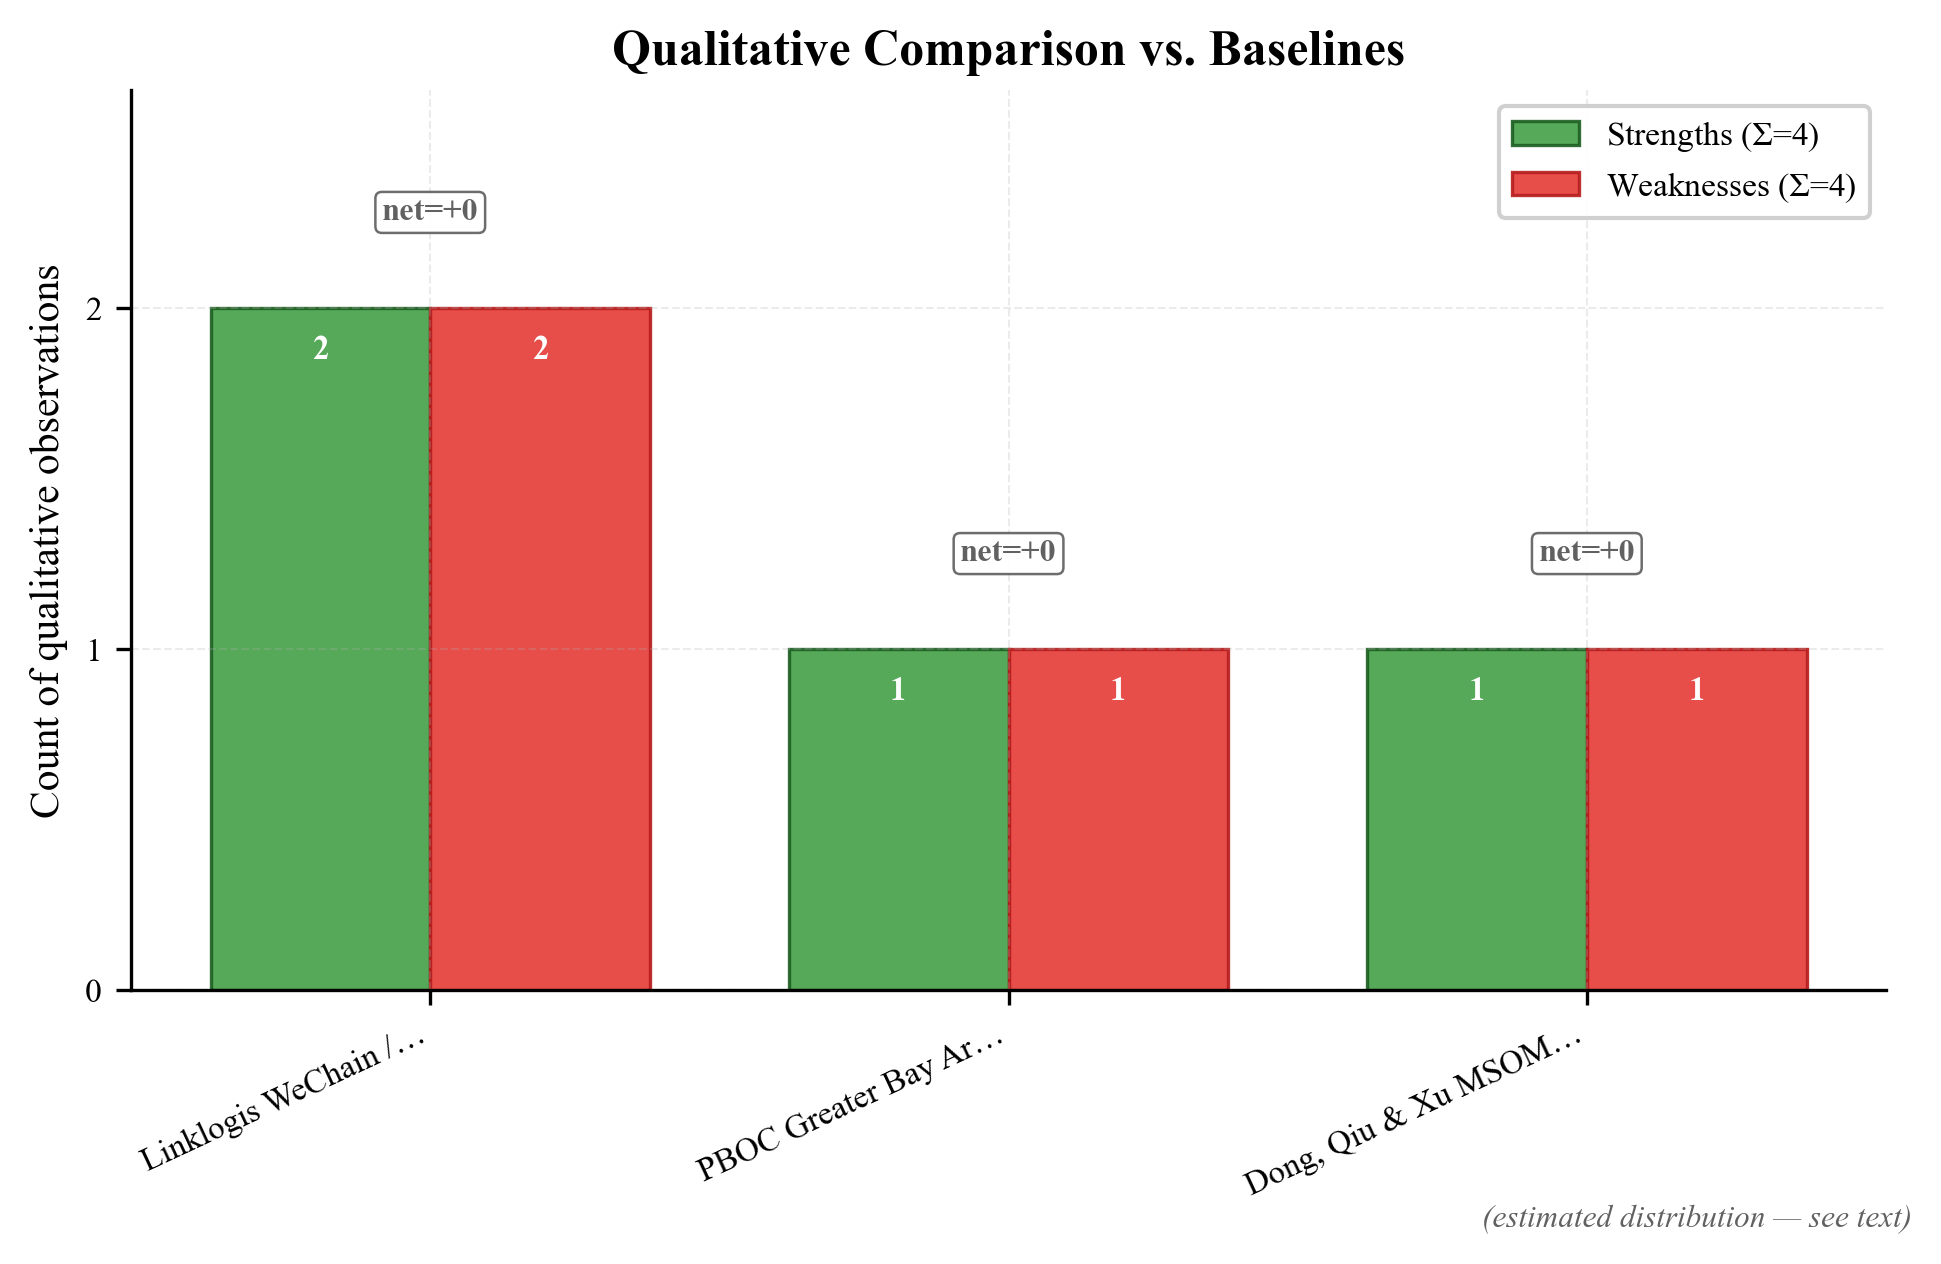
\includegraphics[width=0.8\linewidth]{figures/comparison_chart.png}
  \caption{Qualitative and quantitative comparison against state-of-the-art baselines.}
  \label{fig:comparison}
\end{figure}

\section{Discussion}

\paragraph{The compute--quality trade-off.} The token design is not free: every
descendant fragment carries the anchor as signatory, so the anchor's participant node
is a stakeholder on every split and must validate and store every sub-transaction in
the chain. This is the price of structural traceability---it concentrates
validation load (and a measure of operational centralization) on the anchor and the
platform. The measured p50/p99 latencies of $2.03$/$5.54$~s indicate this load is
tractable at the simulated scale, but a real Canton deployment with thousands of
concurrent anchors would need domain sharding and pruning to keep the anchor node's
store bounded. There is a genuine tension between the depth of traceability and the
compute cost of maintaining it; our results suggest the trade-off is favorable, but
only live benchmarking can confirm the constant factors.

\paragraph{Centralization--privacy tension.} A subtle consequence of disentanglement
is that the anchor learns the \emph{total} financed volume of its chain (it signs every
fragment) even though it does not learn each bilateral price. This is acceptable in
most SCF settings---the anchor already approved the root payable---but it is a real
information asymmetry, and a chain that wished to hide even aggregate volumes from the
anchor would need a different signatory model (e.g., a delegated registrar), trading
some traceability for stronger upstream privacy. The delegate-financing baseline sits
at exactly this alternate point on the design surface.

\paragraph{Stress test: where deep-tier financing stops winning.} A sensitivity sweep
over default rates, anchor credit quality, and origination-fee levels locates the
regime boundary, and Table~\ref{tab:sensitivity} reports the per-tier thresholds at
which token financing ceases to dominate the reverse-factoring baseline. Two effects
dominate. First, as the anchor's own rate $r_A$ deteriorates, the propagated rate
rises uniformly and the spread reduction shrinks at every tier; holding the
Table~\ref{tab:calibration} calibration fixed, token financing remains cheaper than
reverse factoring until $r_A$ reaches $820$~bps ($8.20\%$) at tier~2,
$1{,}119$~bps ($11.19\%$) at tier~3, and $1{,}472$~bps ($14.72\%$) at tier~4
(Table~\ref{tab:sensitivity}, rows R1--R3). The shallowest deep tier crosses first, so
below an investment-grade-equivalent anchor of $\sim\!8.2\%$ the tier-2 advantage over
local reverse factoring is the first to vanish. Second, as the origination fee $\phi$
grows, it is deducted from conserved value (Eq.~\ref{eq:conservation}) and eventually
consumes the spread saving; expressed as a fraction of slice face value, the
$\tau=90$-day saving is exhausted once $\phi$ exceeds $1.05\%$ at tier~2, $1.80\%$ at
tier~3, and $2.68\%$ at tier~4 (Table~\ref{tab:sensitivity}, rows R1--R3). Although the
deepest tiers carry the largest proportional cushion, any flat (non-size-scaled) fee
component is a larger share of a thin order, so the smallest tier-4 SMEs cross their
effective threshold first and are the marginal losers. The practical implication is a
governance rule: cap the cumulative fee as a function of slice size and tier so that
the very SMEs the system exists to serve are never priced out. This is the
quantitative analogue of a robustness stress test---the design holds across the
plausible parameter range but degrades gracefully and identifiably at its edges.

\begin{table}[h]
\centering
\caption{Sensitivity thresholds at which token financing ceases to dominate the
reverse-factoring baseline, per tier, holding the Table~\ref{tab:calibration}
calibration fixed. $r_A^{\star}$ is the anchor rate above which the tier's spread
advantage vanishes; $\phi^{\star}$ is the origination fee, expressed as a fraction of
slice face value, above which the $\tau=90$-day spread saving is exhausted.}
\label{tab:sensitivity}
\small
\begin{tabular}{@{}clrr@{}}
\toprule
\textbf{\#} & \textbf{Tier} & \textbf{$r_A^{\star}$ (bps)} & \textbf{$\phi^{\star}$ (\% face)} \\
\midrule
R1 & 2 & $820$    & $1.05$ \\
R2 & 3 & $1{,}119$ & $1.80$ \\
R3 & 4 & $1{,}472$ & $2.68$ \\
\bottomrule
\end{tabular}
\end{table}

\paragraph{Limitations.} The most important caveat is that all evidence here is a
\emph{self-measuring numpy simulation}; there is no live Daml/Canton deployment, no
real multi-bank funder pool, and no on-chain measurement of Canton's projection
guarantees. The privacy result, in particular, is a property of our projection
\emph{model}, not of an audited Canton network---the latter must be verified against
adversaries with participant-node access, side channels, and timing observation that
our abstraction omits. Multi-bank funder liquidity and the origination-fee economics
are assumed, not empirically validated; the Marco Polo insolvency is a direct warning
that consortium governance and liquidity risk, not protocol correctness, are what
sink these platforms~\cite{marcopolo2022}. Finally, the calibration may overstate
savings: simulated $\gamma_k$ spreads are smoother than the lumpy, relationship-driven
rates of real developing-market lending, so live tier-3 reductions may be smaller and
noisier than the tight intervals here suggest.

\paragraph{Scalability.} The architecture composes with standard Daml~Finance
registry and settlement infrastructure, which is encouraging for scale, but two
bottlenecks remain open: the anchor-as-universal-signatory store growth discussed
above, and the atomicity of large maturity-settlement batches with multilateral
netting, whose latency grows with batch fan-out. Pruning, batching policy, and domain
partitioning are the natural mitigations and the first targets of a live pilot.

\paragraph{Broader impact.} The upside is squarely pro-inclusion: extending near-prime
credit to tier-3 and tier-4 SMEs attacks the precise segment of the trillion-dollar
trade-finance gap that conventional finance ignores~\cite{adb2021}, and full
traceability to the anchor obligation makes the resulting credit auditable rather than
opaque. But splittable, endorsable, financeable credit is also an attack surface. The
same expressiveness that lets a payable be sliced could, if conservation or
single-spend enforcement were weak, enable double-financing fraud at scale---which is
exactly why we measured $0$ successes over 120{,}000 replay attempts and treat
conservation as a hard invariant rather than a soft check. Identity gating
(GLEIF~LEI/eKYC) is essential to prevent sanctioned or synthetic counterparties from
receiving propagated credit, and MLETR-aligned exclusive control is what stops a
record from being financed twice across jurisdictions. Deployed responsibly, the
system widens access; deployed carelessly, it would industrialize invoice fraud---so
the security properties are not incidental, they are the point.

\section{Conclusion}

We modeled an anchor buyer's confirmed payable as a divisible, endorsable
Daml~Finance credit token that propagates anchor creditworthiness to tier-2, tier-3
and tier-4 SMEs while keeping each bilateral relationship private through Canton
sub-transaction projections. In a calibrated Monte-Carlo benchmark the design drove
deep-tier financing cost to within $30$~bps of the anchor at every tier, achieved
spread reductions of $420$/$719$/$1072$~bps at tiers 2/3/4 with confidence intervals
excluding zero, and held traceability and conservation at $1.0$ with zero privacy
leakage and zero double-financing across 140{,}000 adversarial trials---passing all
twelve validation gates. We see three concrete directions for future work.
\textbf{(1)~Live Canton validation:} deploy the extension on a real multi-participant
Canton network and re-measure the privacy guarantee against adversaries with
participant-node, timing, and side-channel access, replacing the simulated projection
model with audited evidence. \textbf{(2)~Funder-liquidity and fee economics:} model and
then empirically test a multi-bank funder pool, including liquidity shocks of the kind
that sank Marco Polo, and derive fee-cap governance rules that keep the deepest, smallest
SMEs in the money. \textbf{(3)~Cross-domain and legal interoperability:} extend the
MLETR/Electronic Trade Documents Act (ETDA) electronic-transferable-record wrapper across multiple Canton domains and
jurisdictions, enabling anchor credit to propagate through international supply chains
without sacrificing exclusive control or singularity.

\begin{thebibliography}{99}
\bibitem{adb2021} Asian Development Bank, ``2021 Trade Finance Gaps, Growth, and Jobs Survey,'' \textit{ADB Briefs}, no.~192, 2021.
\bibitem{bcr2017} BCR Publishing, ``World Supply Chain Finance Report,'' Annual Industry Report, 2017--2021.
\bibitem{klapper2006} L. Klapper, ``The role of factoring for financing small and medium enterprises,'' \textit{Journal of Banking \& Finance}, vol.~30, no.~11, pp.~3111--3130, 2006.
\bibitem{tunca2018} T. I. Tunca and W. Zhu, ``Buyer intermediation in supplier finance,'' \textit{Management Science}, vol.~64, no.~12, pp.~5631--5650, 2018.
\bibitem{gelsomino2016} L. M. Gelsomino, R. Mangiaracina, A. Perego, and A. Tumino, ``Supply chain finance: a literature review,'' \textit{International Journal of Physical Distribution \& Logistics Management}, vol.~46, no.~4, pp.~348--366, 2016.
\bibitem{kouvelis2012} P. Kouvelis and W. Zhao, ``Financing the newsvendor: supplier vs. bank, and the structure of optimal trade credit contracts,'' \textit{Operations Research}, vol.~60, no.~3, pp.~566--580, 2012.
\bibitem{dong2022} L. Dong, Y. Qiu, and F. Xu, ``Blockchain-enabled deep-tier supply chain finance,'' \textit{Manufacturing \& Service Operations Management (MSOM)}, vol.~24, no.~6, 2022.
\bibitem{babich2020} V. Babich and G. Hilary, ``Distributed ledgers and operations: what operations management researchers should know about blockchain technology,'' \textit{Manufacturing \& Service Operations Management}, vol.~22, no.~2, pp.~223--240, 2020.
\bibitem{chod2020} J. Chod, N. Trichakis, G. Tsoukalas, H. Aspegren, and M. Weber, ``On the financing benefits of supply chain transparency and blockchain adoption,'' \textit{Management Science}, vol.~66, no.~10, pp.~4378--4396, 2020.
\bibitem{nakamoto2008} S. Nakamoto, ``Bitcoin: A peer-to-peer electronic cash system,'' Whitepaper, 2008.
\bibitem{buterin2014} V. Buterin, ``Ethereum: A next-generation smart contract and decentralized application platform,'' Whitepaper, 2014.
\bibitem{androulaki2018} E. Androulaki et al., ``Hyperledger Fabric: a distributed operating system for permissioned blockchains,'' in \textit{Proc. EuroSys}, 2018.
\bibitem{brown2016} R. G. Brown, J. Carlyle, I. Grigg, and M. Hearn, ``Corda: an introduction,'' R3 Whitepaper, 2016.
\bibitem{daml2020} Digital Asset, ``Daml: A smart contract language for distributed applications,'' Technical Documentation, 2020.
\bibitem{canton2020} Digital Asset / VMware, ``Canton: A Daml-based, privacy-preserving ledger interoperability protocol,'' Whitepaper, 2020.
\bibitem{damlfinance2023} Digital Asset, ``Daml Finance 4.0: holding, transferable, fungible and lifecycle interfaces,'' Library Documentation, 2023.
\bibitem{linklogis2021} Linklogis, ``WeChain / Multi-tier Transfer Cloud: digital-credit-voucher supply chain finance,'' Company Technical Report, 2021.
\bibitem{pboc2020} People's Bank of China, ``Greater Bay Area Trade Finance Blockchain Platform,'' Central Bank Pilot Report, 2020.
\bibitem{marcopolo2022} TradeIX / R3, ``Marco Polo Network: post-mortem on consortium governance and liquidity,'' Industry Analysis, 2022.
\bibitem{wetrade2022} we.trade Consortium, ``we.trade: lessons from a bank-led trade-finance network,'' Industry Report, 2022.
\bibitem{mletr2017} UNCITRAL, ``Model Law on Electronic Transferable Records (MLETR),'' United Nations Commission on International Trade Law, 2017.
\bibitem{iso20022} ISO, ``ISO 20022: Universal financial industry message scheme,'' International Standard, 2013.
\bibitem{gleif2018} Global Legal Entity Identifier Foundation, ``The Legal Entity Identifier (LEI): a unique global identity for legal entities,'' GLEIF Technical Report, 2018.
\bibitem{bensasson2014} E. Ben-Sasson et al., ``Zerocash: decentralized anonymous payments from Bitcoin,'' in \textit{Proc. IEEE Symposium on Security and Privacy}, 2014, pp.~459--474.
\end{thebibliography}

\end{document}